\documentclass[12pt,a4paper]{article}
\usepackage{amsmath, amssymb, geometry, booktabs, xcolor, hyperref,
            listings, pgfplots, tcolorbox, enumitem, fancyhdr, tikz, array}
\usepgfplotslibrary{fillbetween}
\geometry{margin=2.5cm}
\pgfplotsset{compat=1.18}
\tcbuselibrary{skins, breakable}

\newtcolorbox{curiositybox}[1]{colback=yellow!10, colframe=orange!80, title=#1, breakable}
\newtcolorbox{infobox}[1]{colback=blue!5, colframe=blue!60, title=#1, breakable}
\newtcolorbox{mistakebox}[1]{colback=red!5, colframe=red!60, title=#1, breakable}
\newtcolorbox{learnbox}[1]{colback=green!5, colframe=green!60, title=#1, breakable}

\pagestyle{fancy}
\fancyhf{}
\lhead{Direct Methods \& Applications}
\rhead{Unit 1 -- LAC}
\cfoot{\thepage}

\title{\textbf{Direct Methods: Cramer's Rule, Matrix Inversion \& Engineering Applications} \\ \large Unit 1 -- Matrix Algebra and Linear Systems}
\author{Department of Mathematics}
\date{\today}

\begin{document}
\maketitle
\tableofcontents
\newpage

%% ============================================================
%% SECTION 1: Real-World Engineering Hook
%% ============================================================
\section{Real-World Engineering Hook}

\begin{curiositybox}{Why Should an Engineer Care?}
Imagine you are designing a six-degree-of-freedom robotic arm for a surgical assistant robot. At every millisecond, the arm's onboard controller must answer the question: ``Given the desired tip velocity, what angular speeds should each joint motor run at?'' The mathematical answer is a matrix equation of the form \(\mathbf{J}\,\dot{\boldsymbol{\theta}} = \mathbf{v}\), where \(\mathbf{J}\) is the \(6 \times 6\) Jacobian matrix. Solving for joint rates \(\dot{\boldsymbol{\theta}}\) requires computing \(\mathbf{J}^{-1}\) in real time --- the Matrix Inversion Method at work in a life-critical system.

Now switch to an electrical engineer designing a three-mesh power distribution network. KVL produces three simultaneous equations in the mesh currents. Cramer's Rule yields the symbolic closed-form expression for each current as a ratio of two determinants, making it easy to see exactly how resistance values affect the result --- a transparency no iterative solver offers.

Finally, a chemical process engineer running a three-reactor plant needs the steady-state concentration in each reactor tank, determined by coupled material balance equations. Setting up \(A\mathbf{x} = \mathbf{b}\) and solving via matrix inversion converts a page of differential equations into a single clean matrix multiply.

These three scenarios share one foundation: \textbf{direct methods for solving linear systems}. Unlike iterative methods, they give exact answers in a predictable number of operations --- the right tool when precision and symbolic insight matter more than raw speed.
\end{curiositybox}

%% ============================================================
%% SECTION 2: Why This Topic Exists
%% ============================================================
\section{Theory vs.\ Real-World Impact}

The table below maps each sub-topic to the engineering domain where it delivers the most decisive value.

\begin{center}
\begin{tabular}{@{}p{3.2cm} p{3.8cm} p{5.8cm}@{}}
\toprule
\textbf{Sub-Topic} & \textbf{Engineering Domain} & \textbf{Consequence of Mastery} \\
\midrule
Cramer's Rule & Circuit analysis, Structural statics & Obtain mesh currents / reaction forces as exact algebraic fractions; diagnose singular systems instantly \\
\addlinespace
Matrix Inversion Method & Robotics, Control systems & Pre-compute \(A^{-1}\) once; solve \(A\mathbf{x}=\mathbf{b}\) for hundreds of load cases with a single matrix--vector multiply \\
\addlinespace
Applications to Eng.\ Systems & Chemical process design, Thermal networks & Translate physical laws (KVL, KCL, material balance) into solvable matrix equations; interpret results with physical units \\
\addlinespace
Gauss Elimination (ref.) & Large FEM models & \(O(n^{3}/3)\) --- the backbone of every large-scale linear solver \\
\addlinespace
Gauss--Seidel (ref.) & Sparse power-flow problems & Iterative; effective when \(A\) is diagonally dominant and too large to store as a dense matrix \\
\bottomrule
\end{tabular}
\end{center}

\begin{learnbox}{Pragmatic Method Selection}
Choose your method based on system size, structure, and whether \(A\) is reused --- be pragmatic. Cramer's Rule for \(n \leq 3\) symbolic work, Matrix Inversion when the same coefficient matrix recurs, Gauss Elimination for \(n > 3\) numerical work, Gauss--Seidel for large sparse systems.
\end{learnbox}

%% ============================================================
%% SECTION 3: Definitions --- 3 Subsections
%% ============================================================
\section{Intuition and Formal Definitions}

\subsection{Cramer's Rule}

Picture the solution \(x_i\) of a linear system as a ratio: the ``weight'' that the right-hand side \(\mathbf{b}\) contributes to variable \(i\), divided by the overall capacity of the system captured by \(\det(A)\). When you replace the \(i\)-th column of \(A\) with \(\mathbf{b}\), the determinant of this new matrix encodes exactly how \(\mathbf{b}\) projects onto the \(i\)-th coordinate direction. Dividing by \(\det(A)\) normalises that projection into the actual solution value.

This rule is beautiful for small systems because every variable is independent: if you only need \(x_2\), compute just \(\det(A_2)/\det(A)\) without touching the other variables.

\begin{infobox}{Cramer's Rule --- Formal Statement}
Let \(A\mathbf{x} = \mathbf{b}\) be an \(n \times n\) system where \(\det(A) \neq 0\).

\textbf{Formula:}
\[
x_i = \frac{\det(A_i)}{\det(A)}, \quad i = 1, 2, \ldots, n
\]
where \(A_i\) is the matrix obtained from \(A\) by replacing the \(i\)-th \textbf{column} with \(\mathbf{b}\).

\textbf{Proof sketch:} Left-multiply \(A\mathbf{x} = \mathbf{b}\) by \(\operatorname{adj}(A)\):
\[
\operatorname{adj}(A) \cdot A \cdot \mathbf{x} = \operatorname{adj}(A) \cdot \mathbf{b}
\implies \det(A) \cdot \mathbf{x} = \operatorname{adj}(A) \cdot \mathbf{b}
\implies x_i = \frac{[\operatorname{adj}(A)\,\mathbf{b}]_i}{\det(A)} = \frac{\det(A_i)}{\det(A)}
\]

\textbf{Conditions:}
\begin{itemize}[noitemsep]
  \item \(A\) must be square (\(n \times n\)).
  \item \(\det(A) \neq 0\) (system must be non-singular).
\end{itemize}

\textbf{Computational cost:} \(O(n \cdot n!)\) --- evaluating \(n+1\) determinants of order \(n\) by expansion is factorial in growth.

\textbf{Limitation:} Impractical for \(n > 3\) in numerical computation. Ideal for:
\begin{itemize}[noitemsep]
  \item \(n = 2\) or \(n = 3\) hand calculations.
  \item Symbolic / parametric analysis where closed-form expressions are needed.
\end{itemize}
\end{infobox}

\textbf{Worked Example (Cramer's Rule, 3$\times$3):}

Solve the system:
\[
2x_1 + x_2 - x_3 = 8, \quad -3x_1 - x_2 + 2x_3 = -11, \quad -2x_1 + x_2 + 2x_3 = -3
\]

\textit{Step 1: Write coefficient matrix and right-hand side.}
\[
A = \begin{pmatrix} 2 & 1 & -1 \\ -3 & -1 & 2 \\ -2 & 1 & 2 \end{pmatrix}, \quad \mathbf{b} = \begin{pmatrix} 8 \\ -11 \\ -3 \end{pmatrix}
\]

\textit{Step 2: Compute \(\det(A)\) by cofactor expansion along row 1.}
\begin{align*}
\det(A) &= 2 \cdot \det\begin{pmatrix}-1&2\\1&2\end{pmatrix}
         - 1 \cdot \det\begin{pmatrix}-3&2\\-2&2\end{pmatrix}
         + (-1) \cdot \det\begin{pmatrix}-3&-1\\-2&1\end{pmatrix} \\
&= 2\bigl[(-1)(2)-(2)(1)\bigr]
  - 1\bigl[(-3)(2)-(2)(-2)\bigr]
  + (-1)\bigl[(-3)(1)-(-1)(-2)\bigr] \\
&= 2(-2-2) - 1(-6+4) + (-1)(-3-2) \\
&= 2(-4) - 1(-2) + (-1)(-5) \\
&= -8 + 2 + 5 = -1
\end{align*}

\textit{Step 3: Form \(A_1\) --- replace column 1 with \(\mathbf{b}\).}
\[
A_1 = \begin{pmatrix} \mathbf{8} & 1 & -1 \\ \mathbf{-11} & -1 & 2 \\ \mathbf{-3} & 1 & 2 \end{pmatrix}
\]
\begin{align*}
\det(A_1) &= 8\bigl[(-1)(2)-(2)(1)\bigr]
            - 1\bigl[(-11)(2)-(2)(-3)\bigr]
            + (-1)\bigl[(-11)(1)-(-1)(-3)\bigr] \\
&= 8(-2-2) - 1(-22+6) + (-1)(-11-3) \\
&= 8(-4) - 1(-16) + (-1)(-14) \\
&= -32 + 16 + 14 = -2
\end{align*}

\textit{Step 4: Form \(A_2\) --- replace column 2 with \(\mathbf{b}\).}
\[
A_2 = \begin{pmatrix} 2 & \mathbf{8} & -1 \\ -3 & \mathbf{-11} & 2 \\ -2 & \mathbf{-3} & 2 \end{pmatrix}
\]
\begin{align*}
\det(A_2) &= 2\bigl[(-11)(2)-(2)(-3)\bigr]
            - 8\bigl[(-3)(2)-(2)(-2)\bigr]
            + (-1)\bigl[(-3)(-3)-(-11)(-2)\bigr] \\
&= 2(-22+6) - 8(-6+4) + (-1)(9-22) \\
&= 2(-16) - 8(-2) + (-1)(-13) \\
&= -32 + 16 + 13 = -3
\end{align*}

\textit{Step 5: Form \(A_3\) --- replace column 3 with \(\mathbf{b}\).}
\[
A_3 = \begin{pmatrix} 2 & 1 & \mathbf{8} \\ -3 & -1 & \mathbf{-11} \\ -2 & 1 & \mathbf{-3} \end{pmatrix}
\]
\begin{align*}
\det(A_3) &= 2\bigl[(-1)(-3)-(-11)(1)\bigr]
            - 1\bigl[(-3)(-3)-(-11)(-2)\bigr]
            + 8\bigl[(-3)(1)-(-1)(-2)\bigr] \\
&= 2(3+11) - 1(9-22) + 8(-3-2) \\
&= 2(14) - 1(-13) + 8(-5) \\
&= 28 + 13 - 40 = 1
\end{align*}

\textit{Step 6: Apply Cramer's Rule.}
\[
x_1 = \frac{\det(A_1)}{\det(A)} = \frac{-2}{-1} = 2, \quad
x_2 = \frac{\det(A_2)}{\det(A)} = \frac{-3}{-1} = 3, \quad
x_3 = \frac{\det(A_3)}{\det(A)} = \frac{1}{-1} = -1
\]

\textit{Step 7: Verify by back-substitution.}
\begin{itemize}[noitemsep]
  \item Row 1: \(2(2)+1(3)+(-1)(-1) = 4+3+1 = 8\) \checkmark
  \item Row 2: \(-3(2)+(-1)(3)+2(-1) = -6-3-2 = -11\) \checkmark
  \item Row 3: \(-2(2)+1(3)+2(-1) = -4+3-2 = -3\) \checkmark
\end{itemize}

\textbf{Solution:} \(x_1 = 2,\ x_2 = 3,\ x_3 = -1\).

%% -----------------------------------------------------------
\subsection{Matrix Inversion Method}

When you face the same structural system under ten different load cases --- same frame, different applied forces --- computing the inverse \(A^{-1}\) once and multiplying \(\mathbf{x} = A^{-1}\mathbf{b}\) for each new \(\mathbf{b}\) is dramatically cheaper than re-running Gaussian elimination ten times. The upfront cost of inversion is repaid immediately at scale.

The key is the adjugate (classical adjoint): a matrix assembled from the signed minors of \(A\), then transposed. Divide by the determinant and you have the inverse.

\begin{infobox}{Matrix Inversion Method --- Formal Statement}
For an \(n \times n\) non-singular matrix \(A\) with \(\det(A) \neq 0\):
\[
A^{-1} = \frac{\operatorname{adj}(A)}{\det(A)}
\]
\textbf{Solution formula:}
\[
\mathbf{x} = A^{-1}\mathbf{b} \quad \text{(left-multiply --- NOT } \mathbf{b} \cdot A^{-1}\text{)}
\]

\textbf{Adjugate construction:}
\begin{enumerate}[noitemsep]
  \item Compute each \textbf{minor} \(M_{ij}\): determinant of the \((n-1)\times(n-1)\) submatrix obtained by deleting row \(i\) and column \(j\).
  \item Compute each \textbf{cofactor}: \(C_{ij} = (-1)^{i+j} M_{ij}\).
  \item Build the \textbf{cofactor matrix} \(C\) with entries \(C_{ij}\).
  \item Take the \textbf{transpose}: \(\operatorname{adj}(A) = C^{T}\).
\end{enumerate}

\textbf{Key properties:}
\begin{itemize}[noitemsep]
  \item \((AB)^{-1} = B^{-1}A^{-1}\) --- order reverses on inversion.
  \item \((A^{T})^{-1} = (A^{-1})^{T}\) --- inversion and transposition commute.
  \item \(\det(A^{-1}) = 1/\det(A)\).
\end{itemize}

\textbf{Non-commutativity warning:} In general \(A^{-1}\mathbf{b} \neq \mathbf{b}\, A^{-1}\) since \(\mathbf{b}\) is a column vector; the product \(\mathbf{b}\, A^{-1}\) is not even dimensionally valid for a column vector.

\textbf{Computational cost:} \(O(n^{3})\) to compute \(A^{-1}\); then only \(O(n^{2})\) per subsequent solve.
\end{infobox}

\textbf{Worked Example (Matrix Inversion, 3$\times$3):}

Solve the 3-mesh circuit system:
\[
2x + y + z = 5, \quad 4x - 6y = -2, \quad -2x + 7y + 2z = 9
\]

\textit{Step 1: Identify} \(A\) and \(\mathbf{b}\).
\[
A = \begin{pmatrix} 2 & 1 & 1 \\ 4 & -6 & 0 \\ -2 & 7 & 2 \end{pmatrix}, \quad \mathbf{b} = \begin{pmatrix} 5 \\ -2 \\ 9 \end{pmatrix}
\]

\textit{Step 2: Compute \(\det(A)\) by cofactor expansion along row 1.}
\begin{align*}
\det(A) &= 2\det\begin{pmatrix}-6&0\\7&2\end{pmatrix}
          - 1\det\begin{pmatrix}4&0\\-2&2\end{pmatrix}
          + 1\det\begin{pmatrix}4&-6\\-2&7\end{pmatrix} \\
&= 2[(-6)(2)-(0)(7)] - 1[(4)(2)-(0)(-2)] + 1[(4)(7)-(-6)(-2)] \\
&= 2(-12-0) - 1(8-0) + 1(28-12) \\
&= 2(-12) - 8 + 16 \\
&= -24 - 8 + 16 = -16
\end{align*}
Since \(\det(A) = -16 \neq 0\), the inverse exists.

\textit{Step 3: Compute all 9 cofactors.}

\(C_{11} = (+1)\det\begin{pmatrix}-6&0\\7&2\end{pmatrix} = (-6)(2)-(0)(7) = -12\)

\(C_{12} = (-1)\det\begin{pmatrix}4&0\\-2&2\end{pmatrix} = -[(4)(2)-(0)(-2)] = -(8) = -8\)

\(C_{13} = (+1)\det\begin{pmatrix}4&-6\\-2&7\end{pmatrix} = (4)(7)-(-6)(-2) = 28-12 = 16\)

\(C_{21} = (-1)\det\begin{pmatrix}1&1\\7&2\end{pmatrix} = -[(1)(2)-(1)(7)] = -[2-7] = 5\)

\(C_{22} = (+1)\det\begin{pmatrix}2&1\\-2&2\end{pmatrix} = (2)(2)-(1)(-2) = 4+2 = 6\)

\(C_{23} = (-1)\det\begin{pmatrix}2&1\\-2&7\end{pmatrix} = -[(2)(7)-(1)(-2)] = -[14+2] = -16\)

\(C_{31} = (+1)\det\begin{pmatrix}1&1\\-6&0\end{pmatrix} = (1)(0)-(1)(-6) = 0+6 = 6\)

\(C_{32} = (-1)\det\begin{pmatrix}2&1\\4&0\end{pmatrix} = -[(2)(0)-(1)(4)] = -[0-4] = 4\)

\(C_{33} = (+1)\det\begin{pmatrix}2&1\\4&-6\end{pmatrix} = (2)(-6)-(1)(4) = -12-4 = -16\)

\textit{Step 4: Build cofactor matrix \(C\) and compute \(\operatorname{adj}(A) = C^{T}\).}
\[
C = \begin{pmatrix} -12 & -8 & 16 \\ 5 & 6 & -16 \\ 6 & 4 & -16 \end{pmatrix}
\implies
\operatorname{adj}(A) = C^{T} = \begin{pmatrix} -12 & 5 & 6 \\ -8 & 6 & 4 \\ 16 & -16 & -16 \end{pmatrix}
\]

\textit{Step 5: Compute \(A^{-1} = \operatorname{adj}(A)/\det(A)\).}
\[
A^{-1} = \frac{1}{-16}\begin{pmatrix} -12 & 5 & 6 \\ -8 & 6 & 4 \\ 16 & -16 & -16 \end{pmatrix}
= \begin{pmatrix} 3/4 & -5/16 & -3/8 \\ 1/2 & -3/8 & -1/4 \\ -1 & 1 & 1 \end{pmatrix}
\]

\textit{Step 6: Multiply \(\mathbf{x} = A^{-1}\mathbf{b}\).}
\begin{align*}
x_1 &= \frac{3}{4}(5) + \left(-\frac{5}{16}\right)(-2) + \left(-\frac{3}{8}\right)(9)
     = \frac{15}{4} + \frac{10}{16} - \frac{27}{8}
     = \frac{60}{16} + \frac{10}{16} - \frac{54}{16}
     = \frac{16}{16} = 1 \\
x_2 &= \frac{1}{2}(5) + \left(-\frac{3}{8}\right)(-2) + \left(-\frac{1}{4}\right)(9)
     = \frac{5}{2} + \frac{6}{8} - \frac{9}{4}
     = \frac{20}{8} + \frac{6}{8} - \frac{18}{8}
     = \frac{8}{8} = 1 \\
x_3 &= (-1)(5) + (1)(-2) + (1)(9)
     = -5 - 2 + 9 = 2
\end{align*}

\textit{Step 7: Verify \(A\mathbf{x} = \mathbf{b}\).}
\begin{itemize}[noitemsep]
  \item Row 1: \(2(1)+1(1)+1(2) = 2+1+2 = 5\) \checkmark
  \item Row 2: \(4(1)+(-6)(1)+0(2) = 4-6 = -2\) \checkmark
  \item Row 3: \(-2(1)+7(1)+2(2) = -2+7+4 = 9\) \checkmark
\end{itemize}

\textbf{Solution:} \(x_1 = 1,\ x_2 = 1,\ x_3 = 2\).

%% -----------------------------------------------------------
\subsection{Applications to Engineering Systems}

All the machinery above --- determinants, inverses, Cramer's Rule --- exists to solve one class of problem that appears everywhere in engineering: ``I have \(n\) unknowns obeying \(n\) physical laws simultaneously. Find them.'' The art is translating physical laws into the matrix equation \(A\mathbf{x} = \mathbf{b}\), then choosing the right solver.

Once you master this translation, electrical circuits, structural frames, chemical reactors, thermal networks, and fluid distribution systems all reduce to the same three lines of algebra.

\begin{infobox}{Engineering Systems Modelling Framework}
\textbf{Step-by-step modelling protocol:}
\begin{enumerate}[noitemsep]
  \item \textbf{Identify unknowns:} mesh currents, node voltages, reaction forces, concentrations, flow rates.
  \item \textbf{Write governing equations:} apply KVL, KCL, Newton's laws, material balance, energy balance --- one equation per unknown.
  \item \textbf{Cast into matrix form:} \(A\mathbf{x} = \mathbf{b}\) where each row is one equation, each column corresponds to one unknown.
  \item \textbf{Select method} using the decision framework (see Section 7).
  \item \textbf{Solve} and \textbf{interpret physically} --- check units, signs (current direction, reaction direction), and magnitudes for reasonableness.
  \item \textbf{Verify:} compute \(A\mathbf{x}\) and confirm it equals \(\mathbf{b}\).
\end{enumerate}

\textbf{Method selection decision framework (preview):}
\begin{center}
\begin{tabular}{@{}lll@{}}
\toprule
\textbf{Situation} & \textbf{Recommended Method} & \textbf{Reason} \\
\midrule
\(n \leq 3\), need symbolic answer & Cramer's Rule & Exact closed form \\
Same \(A\), many \(\mathbf{b}\) vectors & Matrix Inversion & One-time \(O(n^3)\) cost \\
\(n > 3\), single solve & Gauss Elimination & \(O(n^3/3)\) most efficient \\
Large, sparse, diagonally dominant & Gauss--Seidel & Memory-efficient iteration \\
\bottomrule
\end{tabular}
\end{center}
\end{infobox}

\textbf{Worked Example A: 3-Mesh Electrical Circuit (Cramer's Rule)}

A DC circuit has three mesh loops. Applying KVL to each loop yields:
\[
5I_1 - 2I_2 + 0\,I_3 = 10, \quad -2I_1 + 6I_2 - I_3 = 0, \quad 0\,I_1 - I_2 + 4I_3 = 8
\]
where \(I_1, I_2, I_3\) are mesh currents in amperes.

\textit{Step 1: Coefficient matrix and right-hand side.}
\[
A = \begin{pmatrix} 5 & -2 & 0 \\ -2 & 6 & -1 \\ 0 & -1 & 4 \end{pmatrix}, \quad \mathbf{b} = \begin{pmatrix} 10 \\ 0 \\ 8 \end{pmatrix}
\]

\textit{Step 2: Compute \(\det(A)\) expanding along row 1.}
\begin{align*}
\det(A) &= 5\det\begin{pmatrix}6&-1\\-1&4\end{pmatrix}
          - (-2)\det\begin{pmatrix}-2&-1\\0&4\end{pmatrix}
          + 0 \\
&= 5[(6)(4)-(-1)(-1)] + 2[(-2)(4)-(-1)(0)] \\
&= 5[24-1] + 2[-8-0] \\
&= 5(23) + 2(-8) = 115 - 16 = 99
\end{align*}

\textit{Step 3: Form \(A_1\) --- replace column 1 with \(\mathbf{b}\).}
\[
A_1 = \begin{pmatrix} \mathbf{10} & -2 & 0 \\ \mathbf{0} & 6 & -1 \\ \mathbf{8} & -1 & 4 \end{pmatrix}
\]
\begin{align*}
\det(A_1) &= 10\det\begin{pmatrix}6&-1\\-1&4\end{pmatrix}
            - (-2)\det\begin{pmatrix}0&-1\\8&4\end{pmatrix}
            + 0 \\
&= 10[(6)(4)-(-1)(-1)] + 2[(0)(4)-(-1)(8)] \\
&= 10(24-1) + 2(0+8) \\
&= 10(23) + 2(8) = 230 + 16 = 246
\end{align*}

\textit{Step 4: Form \(A_2\) --- replace column 2 with \(\mathbf{b}\).}
\[
A_2 = \begin{pmatrix} 5 & \mathbf{10} & 0 \\ -2 & \mathbf{0} & -1 \\ 0 & \mathbf{8} & 4 \end{pmatrix}
\]
\begin{align*}
\det(A_2) &= 5\det\begin{pmatrix}0&-1\\8&4\end{pmatrix}
            - 10\det\begin{pmatrix}-2&-1\\0&4\end{pmatrix}
            + 0 \\
&= 5[(0)(4)-(-1)(8)] - 10[(-2)(4)-(-1)(0)] \\
&= 5(0+8) - 10(-8-0) \\
&= 40 + 80 = 120
\end{align*}

\textit{Step 5: Form \(A_3\) --- replace column 3 with \(\mathbf{b}\).}
\[
A_3 = \begin{pmatrix} 5 & -2 & \mathbf{10} \\ -2 & 6 & \mathbf{0} \\ 0 & -1 & \mathbf{8} \end{pmatrix}
\]
\begin{align*}
\det(A_3) &= 5\det\begin{pmatrix}6&0\\-1&8\end{pmatrix}
            - (-2)\det\begin{pmatrix}-2&0\\0&8\end{pmatrix}
            + 10\det\begin{pmatrix}-2&6\\0&-1\end{pmatrix} \\
&= 5[(6)(8)-(0)(-1)] + 2[(-2)(8)-(0)(0)] + 10[(-2)(-1)-(6)(0)] \\
&= 5(48) + 2(-16) + 10(2) \\
&= 240 - 32 + 20 = 228
\end{align*}

\textit{Step 6: Apply Cramer's Rule.}
\[
I_1 = \frac{246}{99} = \frac{82}{33} \approx 2.485\,\text{A}, \quad
I_2 = \frac{120}{99} = \frac{40}{33} \approx 1.212\,\text{A}, \quad
I_3 = \frac{228}{99} = \frac{76}{33} \approx 2.303\,\text{A}
\]

\textit{Step 7: Verify.}
\begin{itemize}[noitemsep]
  \item Row 1: \(5\!\cdot\!\tfrac{82}{33} - 2\!\cdot\!\tfrac{40}{33} = \tfrac{410-80}{33} = \tfrac{330}{33} = 10\) \checkmark
  \item Row 2: \(-2\!\cdot\!\tfrac{82}{33} + 6\!\cdot\!\tfrac{40}{33} - \tfrac{76}{33} = \tfrac{-164+240-76}{33} = \tfrac{0}{33} = 0\) \checkmark
  \item Row 3: \(-\tfrac{40}{33} + 4\!\cdot\!\tfrac{76}{33} = \tfrac{-40+304}{33} = \tfrac{264}{33} = 8\) \checkmark
\end{itemize}

\textit{Power at the 10\,V source:} \(P = V \cdot I_1 = 10 \times \tfrac{82}{33} \approx 24.85\,\text{W}\).

\medskip
\textbf{Worked Example B: 3-Reactor Chemical Plant (Matrix Inversion)}

Three continuous stirred-tank reactors (CSTRs) are connected in series. A steady-state material balance around each reactor yields:
\[
3C_1 - C_2 + 0\,C_3 = 10, \quad -C_1 + 4C_2 - C_3 = 5, \quad 0\,C_1 - C_2 + 3C_3 = 8
\]
where \(C_1, C_2, C_3\) are concentrations in mol/L.

\textit{Step 1: Form \(A\) and \(\mathbf{b}\).}
\[
A = \begin{pmatrix} 3 & -1 & 0 \\ -1 & 4 & -1 \\ 0 & -1 & 3 \end{pmatrix}, \quad \mathbf{b} = \begin{pmatrix} 10 \\ 5 \\ 8 \end{pmatrix}
\]

\textit{Step 2: Compute \(\det(A)\).}
\begin{align*}
\det(A) &= 3\det\begin{pmatrix}4&-1\\-1&3\end{pmatrix}
          - (-1)\det\begin{pmatrix}-1&-1\\0&3\end{pmatrix}
          + 0 \\
&= 3[(4)(3)-(-1)(-1)] + 1[(-1)(3)-(-1)(0)] \\
&= 3(12-1) + 1(-3-0) \\
&= 3(11) - 3 = 33 - 3 = 30
\end{align*}

\textit{Step 3: Compute all 9 cofactors.}

\(C_{11} = (+1)\det\begin{pmatrix}4&-1\\-1&3\end{pmatrix} = 12-1 = 11\)

\(C_{12} = (-1)\det\begin{pmatrix}-1&-1\\0&3\end{pmatrix} = -[(-1)(3)-(-1)(0)] = -(-3) = 3\)

\(C_{13} = (+1)\det\begin{pmatrix}-1&4\\0&-1\end{pmatrix} = (-1)(-1)-(4)(0) = 1\)

\(C_{21} = (-1)\det\begin{pmatrix}-1&0\\-1&3\end{pmatrix} = -[(-1)(3)-(0)(-1)] = -(-3) = 3\)

\(C_{22} = (+1)\det\begin{pmatrix}3&0\\0&3\end{pmatrix} = (3)(3)-(0)(0) = 9\)

\(C_{23} = (-1)\det\begin{pmatrix}3&-1\\0&-1\end{pmatrix} = -[(3)(-1)-(-1)(0)] = -(-3) = 3\)

\(C_{31} = (+1)\det\begin{pmatrix}-1&0\\4&-1\end{pmatrix} = (-1)(-1)-(0)(4) = 1\)

\(C_{32} = (-1)\det\begin{pmatrix}3&0\\-1&-1\end{pmatrix} = -[(3)(-1)-(0)(-1)] = -(-3) = 3\)

\(C_{33} = (+1)\det\begin{pmatrix}3&-1\\-1&4\end{pmatrix} = (3)(4)-(-1)(-1) = 12-1 = 11\)

\textit{Step 4: Build \(\operatorname{adj}(A) = C^{T}\).}
\[
C = \begin{pmatrix}11&3&1\\3&9&3\\1&3&11\end{pmatrix}
\implies
\operatorname{adj}(A) = \begin{pmatrix}11&3&1\\3&9&3\\1&3&11\end{pmatrix}
\]
(Note: this cofactor matrix is symmetric, so \(\operatorname{adj}(A)=C^{T}=C\) here.)

\textit{Step 5: Compute \(A^{-1}\).}
\[
A^{-1} = \frac{1}{30}\begin{pmatrix}11&3&1\\3&9&3\\1&3&11\end{pmatrix}
\]

\textit{Step 6: Multiply \(\mathbf{x} = A^{-1}\mathbf{b}\).}
\begin{align*}
C_1 &= \frac{1}{30}\bigl[11(10)+3(5)+1(8)\bigr] = \frac{110+15+8}{30} = \frac{133}{30} \approx 4.43\,\text{mol/L} \\
C_2 &= \frac{1}{30}\bigl[3(10)+9(5)+3(8)\bigr] = \frac{30+45+24}{30} = \frac{99}{30} = 3.30\,\text{mol/L} \\
C_3 &= \frac{1}{30}\bigl[1(10)+3(5)+11(8)\bigr] = \frac{10+15+88}{30} = \frac{113}{30} \approx 3.77\,\text{mol/L}
\end{align*}

\textit{Step 7: Verify \(A\mathbf{x} = \mathbf{b}\).}
\begin{itemize}[noitemsep]
  \item Row 1: \(3\!\cdot\!\tfrac{133}{30} - \tfrac{99}{30} = \tfrac{399-99}{30} = \tfrac{300}{30} = 10\) \checkmark
  \item Row 2: \(-\tfrac{133}{30} + 4\!\cdot\!\tfrac{99}{30} - \tfrac{113}{30} = \tfrac{-133+396-113}{30} = \tfrac{150}{30} = 5\) \checkmark
  \item Row 3: \(-\tfrac{99}{30} + 3\!\cdot\!\tfrac{113}{30} = \tfrac{-99+339}{30} = \tfrac{240}{30} = 8\) \checkmark
\end{itemize}

\textit{Physical interpretation:} Reactor 1 has the highest concentration (\(\approx 4.43\) mol/L) as it receives the feed stream directly. Each downstream reactor shows lower concentration due to reaction conversion. All concentrations are positive, confirming physical validity.

%% ============================================================
%% SECTION 4: Visual Artifacts
%% ============================================================
\section{Visual Artifacts}

\subsection*{Visual 1: Cramer's Rule --- Column Replacement Diagram}

\begin{center}
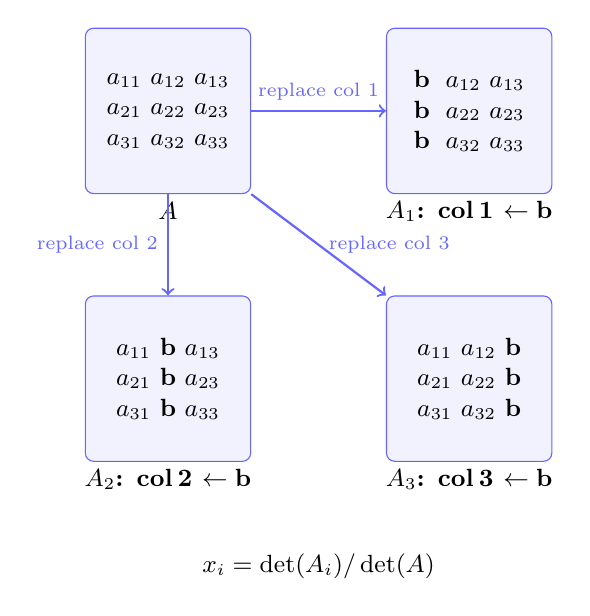
\begin{tikzpicture}[scale=0.85,
  matbox/.style={draw=blue!60, fill=blue!5, rounded corners=3pt, minimum width=2.1cm, minimum height=2.1cm, align=center, font=\small},
  bvec/.style={draw=orange!80, fill=orange!20, rounded corners=3pt, minimum width=0.55cm, minimum height=2.1cm, align=center, font=\small\bfseries},
  lbl/.style={font=\small\bfseries, align=center}
]
% Original A
\node[matbox] (A) at (0,0) {$a_{11}\ a_{12}\ a_{13}$\\$a_{21}\ a_{22}\ a_{23}$\\$a_{31}\ a_{32}\ a_{33}$};
\node[lbl] at (0,-1.5) {$A$};

% A1
\node[matbox] (A1) at (4.5,0) {$\mathbf{b}\ \; a_{12}\ a_{13}$\\$\mathbf{b}\ \; a_{22}\ a_{23}$\\$\mathbf{b}\ \; a_{32}\ a_{33}$};
\node[lbl] at (4.5,-1.5) {$A_1$: col\,1 $\leftarrow \mathbf{b}$};

% A2
\node[matbox] (A2) at (0,-4) {$a_{11}\ \mathbf{b}\ a_{13}$\\$a_{21}\ \mathbf{b}\ a_{23}$\\$a_{31}\ \mathbf{b}\ a_{33}$};
\node[lbl] at (0,-5.5) {$A_2$: col\,2 $\leftarrow \mathbf{b}$};

% A3
\node[matbox] (A3) at (4.5,-4) {$a_{11}\ a_{12}\ \mathbf{b}$\\$a_{21}\ a_{22}\ \mathbf{b}$\\$a_{31}\ a_{32}\ \mathbf{b}$};
\node[lbl] at (4.5,-5.5) {$A_3$: col\,3 $\leftarrow \mathbf{b}$};

% Arrows from A
\draw[->, thick, blue!60] (A.east) -- (A1.west) node[midway, above, font=\scriptsize] {replace col 1};
\draw[->, thick, blue!60] (A.south) -- (A2.north) node[midway, left, font=\scriptsize] {replace col 2};
\draw[->, thick, blue!60] (A.south east) -- (A3.north west) node[midway, right, font=\scriptsize] {replace col 3};

% Formula labels
\node[font=\small] at (2.25,-6.8) {$x_i = \det(A_i)/\det(A)$};
\end{tikzpicture}
\end{center}

\subsection*{Visual 2: Matrix Inversion Pipeline Flowchart}

\begin{center}
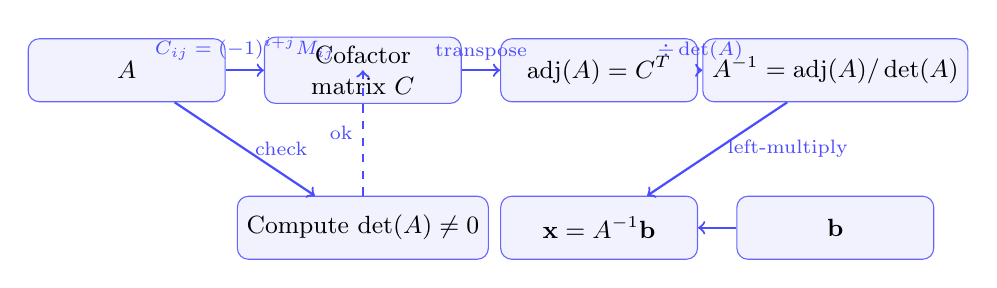
\begin{tikzpicture}[
  box/.style={draw=blue!60, fill=blue!5, rounded corners=4pt, minimum width=2.5cm, minimum height=0.8cm, align=center, font=\small},
  arr/.style={->, thick, blue!70}
]
\node[box] (A)    at (0,0)   {$A$};
\node[box] (Cof)  at (3,0)   {Cofactor\\matrix $C$};
\node[box] (Adj)  at (6,0)   {$\operatorname{adj}(A)=C^T$};
\node[box] (Inv)  at (9,0)   {$A^{-1}=\operatorname{adj}(A)/\det(A)$};
\node[box] (b)    at (9,-2)  {$\mathbf{b}$};
\node[box] (x)    at (6,-2)  {$\mathbf{x}=A^{-1}\mathbf{b}$};
\node[box] (det)  at (3,-2)  {Compute $\det(A)\neq 0$};

\draw[arr] (A)   -- (Cof)  node[midway,above,font=\scriptsize]{$C_{ij}=(-1)^{i+j}M_{ij}$};
\draw[arr] (Cof) -- (Adj)  node[midway,above,font=\scriptsize]{transpose};
\draw[arr] (Adj) -- (Inv)  node[midway,above,font=\scriptsize]{$\div\det(A)$};
\draw[arr] (Inv) -- (x)    node[midway,right,font=\scriptsize]{left-multiply};
\draw[arr] (b)   -- (x);
\draw[arr] (A)   -- (det)  node[midway,right,font=\scriptsize]{check};
\draw[arr,dashed] (det) -- (3,0) node[midway,left,font=\scriptsize]{ok};
\end{tikzpicture}
\end{center}

\subsection*{Visual 3: Computational Operations --- Method Comparison (pgfplots)}

\begin{center}
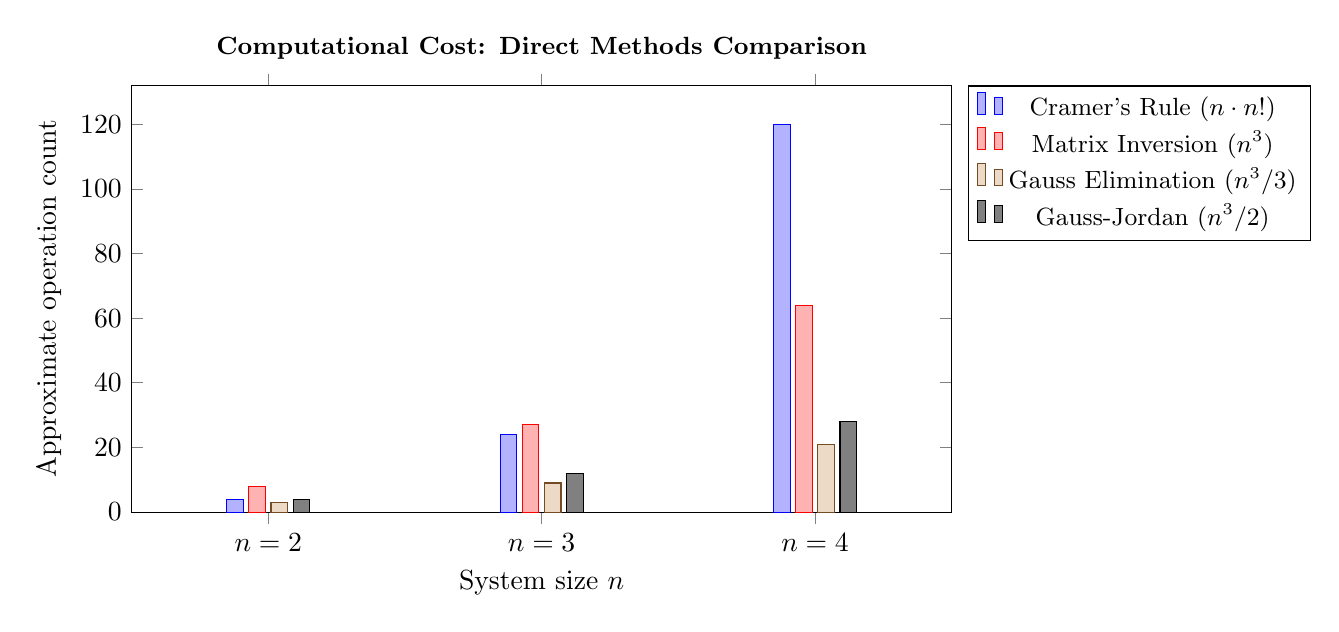
\begin{tikzpicture}
\begin{axis}[
  ybar,
  bar width=6pt,
  width=12cm, height=7cm,
  xlabel={System size $n$},
  ylabel={Approximate operation count},
  xtick={2,3,4},
  xticklabels={$n=2$, $n=3$, $n=4$},
  legend style={at={(1.02,1)}, anchor=north west, font=\small},
  ymin=0,
  enlarge x limits=0.25,
  title={Computational Cost: Direct Methods Comparison},
  title style={font=\small\bfseries}
]
\addplot coordinates {(2,4) (3,24) (4,120)};
\addlegendentry{Cramer's Rule ($n\cdot n!$)}
\addplot coordinates {(2,8) (3,27) (4,64)};
\addlegendentry{Matrix Inversion ($n^3$)}
\addplot coordinates {(2,3) (3,9) (4,21)};
\addlegendentry{Gauss Elimination ($n^3/3$)}
\addplot coordinates {(2,4) (3,12) (4,28)};
\addlegendentry{Gauss-Jordan ($n^3/2$)}
\end{axis}
\end{tikzpicture}
\end{center}

\subsection*{Visual 4: 3-Mesh Circuit Diagram}

\begin{center}
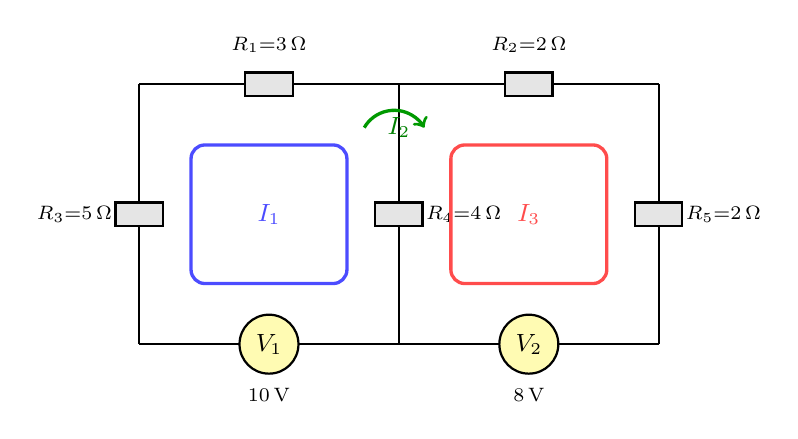
\begin{tikzpicture}[scale=1.1,
  comp/.style={draw, thick, minimum width=0.6cm, minimum height=0.3cm, fill=gray!20},
  wire/.style={thick},
  vsrc/.style={draw, circle, thick, fill=yellow!30, minimum size=0.7cm, font=\small}
]
% Outer rectangle (Mesh 1 top, Mesh 3 bottom)
% Top-left corner
\coordinate (TL) at (0,3);
\coordinate (TR) at (6,3);
\coordinate (BL) at (0,0);
\coordinate (BR) at (6,0);
\coordinate (TM) at (3,3);
\coordinate (BM) at (3,0);

% Draw wires
\draw[wire] (TL) -- (TM);
\draw[wire] (TM) -- (TR);
\draw[wire] (BL) -- (BM);
\draw[wire] (BM) -- (BR);
\draw[wire] (TL) -- (BL);
\draw[wire] (TR) -- (BR);
\draw[wire] (TM) -- (BM);

% R1 on top-left segment
\node[comp] (R1) at (1.5, 3) {};
\node[above, font=\scriptsize] at (1.5,3.25) {$R_1{=}3\,\Omega$};

% R2 on top-right segment
\node[comp] (R2) at (4.5, 3) {};
\node[above, font=\scriptsize] at (4.5,3.25) {$R_2{=}2\,\Omega$};

% R3 on left side
\node[comp] (R3) at (0, 1.5) {};
\node[left, font=\scriptsize] at (-0.2,1.5) {$R_3{=}5\,\Omega$};

% R4 on middle
\node[comp] (R4) at (3, 1.5) {};
\node[right, font=\scriptsize] at (3.2,1.5) {$R_4{=}4\,\Omega$};

% R5 on right side
\node[comp] (R5) at (6, 1.5) {};
\node[right, font=\scriptsize] at (6.2,1.5) {$R_5{=}2\,\Omega$};

% V1 on bottom-left
\node[vsrc] at (1.5, 0) {$V_1$};
\node[below, font=\scriptsize] at (1.5,-0.4) {$10\,\text{V}$};

% V2 on bottom-right
\node[vsrc] at (4.5, 0) {$V_2$};
\node[below, font=\scriptsize] at (4.5,-0.4) {$8\,\text{V}$};

% Mesh current arrows
\draw[->, very thick, blue!70, rounded corners=5pt]
  (0.6,2.3) -- (2.4,2.3) -- (2.4,0.7) -- (0.6,0.7) -- cycle;
\node[blue!70, font=\small\bfseries] at (1.5,1.5) {$I_1$};

\draw[->, very thick, red!70, rounded corners=5pt]
  (3.6,2.3) -- (5.4,2.3) -- (5.4,0.7) -- (3.6,0.7) -- cycle;
\node[red!70, font=\small\bfseries] at (4.5,1.5) {$I_3$};

% Middle mesh (I2 through shared branch implied)
\node[green!50!black, font=\small\bfseries] at (3,2.5) {$I_2$};
\draw[->, very thick, green!60!black] (2.6,2.5) arc(150:30:0.4);
\end{tikzpicture}
\end{center}

%% ============================================================
%% SECTION 5: Step-by-Step Algorithmic Workflows
%% ============================================================
\section{Step-by-Step Algorithmic Workflows}

\begin{learnbox}{Algorithm 1: Cramer's Rule}
\begin{enumerate}[noitemsep]
  \item Write the system as \(A\mathbf{x} = \mathbf{b}\) with \(A\) a square \(n\times n\) matrix.
  \item Compute \(D = \det(A)\). \textbf{If \(D = 0\), stop} --- the system is singular (no unique solution).
  \item For each \(i = 1, 2, \ldots, n\):
  \begin{enumerate}[noitemsep, label=\alph*.]
    \item Form \(A_i\) by replacing \textbf{column} \(i\) of \(A\) with \(\mathbf{b}\) (not row \(i\)).
    \item Compute \(D_i = \det(A_i)\) by cofactor expansion.
    \item Set \(x_i = D_i / D\).
  \end{enumerate}
  \item Verify: substitute \(\mathbf{x}\) into \(A\mathbf{x}\) and confirm the result equals \(\mathbf{b}\).
\end{enumerate}
\end{learnbox}

\begin{learnbox}{Algorithm 2: Matrix Inversion Method}
\begin{enumerate}[noitemsep]
  \item Write \(A\mathbf{x} = \mathbf{b}\).
  \item Compute \(D = \det(A)\). \textbf{If \(D = 0\), stop} --- \(A\) is not invertible.
  \item For each entry \((i,j)\): compute the minor \(M_{ij}\) (determinant of the \((n-1)\times(n-1)\) submatrix by deleting row \(i\) and column \(j\)).
  \item Compute cofactor: \(C_{ij} = (-1)^{i+j} M_{ij}\).
  \item Assemble cofactor matrix \(C = [C_{ij}]\).
  \item Compute adjugate: \(\operatorname{adj}(A) = C^{T}\) (transpose the cofactor matrix).
  \item Compute inverse: \(A^{-1} = \operatorname{adj}(A) / D\).
  \item Multiply: \(\mathbf{x} = A^{-1}\mathbf{b}\) (left-multiply).
  \item Verify: compute \(A\mathbf{x}\) and confirm it equals \(\mathbf{b}\).
\end{enumerate}
\end{learnbox}

\begin{learnbox}{Algorithm 3: Engineering Modelling Protocol}
\begin{enumerate}[noitemsep]
  \item \textbf{Identify unknowns:} List all quantities to be found (e.g., mesh currents, node temperatures, concentrations). Count them --- this is \(n\).
  \item \textbf{Write governing equations:} Apply one physical law per unknown --- KVL for circuits, Newton's law for statics, mass balance for chemistry.
  \item \textbf{Standardise each equation:} Move all unknown terms to the left, constants to the right. Align unknowns by column position.
  \item \textbf{Form \(A\mathbf{x} = \mathbf{b}\):} Each row of \(A\) holds the coefficients from one equation; \(\mathbf{b}\) holds the right-hand side constants.
  \item \textbf{Select solver:} Use the decision table (Section 7) based on \(n\), structure of \(A\), and whether multiple \(\mathbf{b}\) vectors will be needed.
  \item \textbf{Solve} using the chosen algorithm.
  \item \textbf{Interpret physically:} Check units, confirm sign conventions (e.g., negative current means opposite direction), verify magnitudes are physically reasonable.
  \item \textbf{Verify:} Compute \(A\mathbf{x}\) and confirm equality with \(\mathbf{b}\) --- never skip this step.
\end{enumerate}
\end{learnbox}

%% ============================================================
%% SECTION 6: Fully Worked Numerical Examples
%% ============================================================
\section{Fully Worked Numerical Examples}

\subsection*{Example 1: Cramer's Rule (2$\times$2)}

Solve: \(3x + 2y = 7,\quad x - y = 1\).

\textit{Step 1: Coefficient matrix.}
\[
A = \begin{pmatrix} 3 & 2 \\ 1 & -1 \end{pmatrix}, \quad \mathbf{b} = \begin{pmatrix} 7 \\ 1 \end{pmatrix}
\]

\textit{Step 2:} \(\det(A) = (3)(-1) - (2)(1) = -3 - 2 = -5\).

\textit{Step 3: Form \(A_1\) --- replace column 1 with \(\mathbf{b}\).}
\[
A_1 = \begin{pmatrix} \mathbf{7} & 2 \\ \mathbf{1} & -1 \end{pmatrix}, \quad \det(A_1) = (7)(-1)-(2)(1) = -7-2 = -9
\]

\textit{Step 4: Form \(A_2\) --- replace column 2 with \(\mathbf{b}\).}
\[
A_2 = \begin{pmatrix} 3 & \mathbf{7} \\ 1 & \mathbf{1} \end{pmatrix}, \quad \det(A_2) = (3)(1)-(7)(1) = 3-7 = -4
\]

\textit{Step 5: Apply Cramer's Rule.}
\[
x = \frac{-9}{-5} = \frac{9}{5} = 1.8, \quad y = \frac{-4}{-5} = \frac{4}{5} = 0.8
\]

\textit{Step 6: Verify.}
\begin{itemize}[noitemsep]
  \item \(3(1.8)+2(0.8) = 5.4+1.6 = 7\) \checkmark
  \item \(1.8 - 0.8 = 1\) \checkmark
\end{itemize}

\begin{learnbox}{Insight}
For \(2\times2\) systems, Cramer's Rule is the fastest hand-calculation method --- only two \(2\times2\) determinants needed.
\end{learnbox}

\subsection*{Example 2: Cramer's Rule (3$\times$3, Full)}

Solve: \(x + 2y - z = 6,\quad 2x + y + 3z = 14,\quad -x + 3y - 2z = 2\).

\textit{Step 1:}
\[
A = \begin{pmatrix}1&2&-1\\2&1&3\\-1&3&-2\end{pmatrix}, \quad \mathbf{b} = \begin{pmatrix}6\\14\\2\end{pmatrix}
\]

\textit{Step 2: Compute \(\det(A)\) expanding along row 1.}
\begin{align*}
\det(A) &= 1\det\begin{pmatrix}1&3\\3&-2\end{pmatrix}
          - 2\det\begin{pmatrix}2&3\\-1&-2\end{pmatrix}
          + (-1)\det\begin{pmatrix}2&1\\-1&3\end{pmatrix} \\
&= 1[(1)(-2)-(3)(3)] - 2[(2)(-2)-(3)(-1)] + (-1)[(2)(3)-(1)(-1)] \\
&= 1(-2-9) - 2(-4+3) + (-1)(6+1) \\
&= 1(-11) - 2(-1) - 1(7) \\
&= -11 + 2 - 7 = -16
\end{align*}

\textit{Step 3: Form \(A_1\) --- replace column 1 with \(\mathbf{b}\).}
\[
A_1 = \begin{pmatrix}\mathbf{6}&2&-1\\\mathbf{14}&1&3\\\mathbf{2}&3&-2\end{pmatrix}
\]
\begin{align*}
\det(A_1) &= 6\det\begin{pmatrix}1&3\\3&-2\end{pmatrix}
            - 2\det\begin{pmatrix}14&3\\2&-2\end{pmatrix}
            + (-1)\det\begin{pmatrix}14&1\\2&3\end{pmatrix} \\
&= 6(-2-9) - 2(-28-6) + (-1)(42-2) \\
&= 6(-11) - 2(-34) - 1(40) \\
&= -66 + 68 - 40 = -38
\end{align*}

\textit{Step 4: Form \(A_2\) --- replace column 2 with \(\mathbf{b}\).}
\[
A_2 = \begin{pmatrix}1&\mathbf{6}&-1\\2&\mathbf{14}&3\\-1&\mathbf{2}&-2\end{pmatrix}
\]
\begin{align*}
\det(A_2) &= 1\det\begin{pmatrix}14&3\\2&-2\end{pmatrix}
            - 6\det\begin{pmatrix}2&3\\-1&-2\end{pmatrix}
            + (-1)\det\begin{pmatrix}2&14\\-1&2\end{pmatrix} \\
&= 1(-28-6) - 6(-4+3) + (-1)(4+14) \\
&= 1(-34) - 6(-1) + (-1)(18) \\
&= -34 + 6 - 18 = -46
\end{align*}

\textit{Step 5: Form \(A_3\) --- replace column 3 with \(\mathbf{b}\).}
\[
A_3 = \begin{pmatrix}1&2&\mathbf{6}\\2&1&\mathbf{14}\\-1&3&\mathbf{2}\end{pmatrix}
\]
\begin{align*}
\det(A_3) &= 1\det\begin{pmatrix}1&14\\3&2\end{pmatrix}
            - 2\det\begin{pmatrix}2&14\\-1&2\end{pmatrix}
            + 6\det\begin{pmatrix}2&1\\-1&3\end{pmatrix} \\
&= 1(2-42) - 2(4+14) + 6(6+1) \\
&= 1(-40) - 2(18) + 6(7) \\
&= -40 - 36 + 42 = -34
\end{align*}

\textit{Step 6: Cramer's Rule.}
\[
x = \frac{-38}{-16} = \frac{19}{8} = 2.375, \quad
y = \frac{-46}{-16} = \frac{23}{8} = 2.875, \quad
z = \frac{-34}{-16} = \frac{17}{8} = 2.125
\]

\textit{Step 7: Verify.}
\begin{itemize}[noitemsep]
  \item Row 1: \(\tfrac{19}{8} + 2\cdot\tfrac{23}{8} - \tfrac{17}{8} = \tfrac{19+46-17}{8} = \tfrac{48}{8} = 6\) \checkmark
  \item Row 2: \(2\cdot\tfrac{19}{8} + \tfrac{23}{8} + 3\cdot\tfrac{17}{8} = \tfrac{38+23+51}{8} = \tfrac{112}{8} = 14\) \checkmark
  \item Row 3: \(-\tfrac{19}{8} + 3\cdot\tfrac{23}{8} - 2\cdot\tfrac{17}{8} = \tfrac{-19+69-34}{8} = \tfrac{16}{8} = 2\) \checkmark
\end{itemize}

\begin{learnbox}{Insight}
For \(3\times3\) systems, Cramer's Rule requires 4 full determinant evaluations --- always check \(\det(A) \neq 0\) first to avoid division by zero.
\end{learnbox}

\subsection*{Example 3: Matrix Inversion (3$\times$3)}

(See the fully worked example in Section 3.2 above --- all 9 cofactors computed individually, adjugate, \(A^{-1}\), and verification.)

\begin{learnbox}{Insight}
Computing \(A^{-1}\) costs more upfront but pays off when solving for multiple \(\mathbf{b}\) vectors --- the one-time investment in inversion saves repeated Gaussian eliminations.
\end{learnbox}

\subsection*{Example 4: Engineering Application --- 3-Mesh Circuit (Cramer's Rule)}

(See Section 3.3, Worked Example A --- KVL gives \(5I_1-2I_2=10\), \(-2I_1+6I_2-I_3=0\), \(-I_2+4I_3=8\). Solution: \(I_1 = 82/33\), \(I_2 = 40/33\), \(I_3 = 76/33\) amperes. Power \(P \approx 24.85\) W.)

\begin{learnbox}{Insight}
Cramer's Rule gives mesh currents as exact fractions --- ideal for symbolic circuit analysis where you need to see how resistance values affect the current algebraically.
\end{learnbox}

\subsection*{Example 5: Engineering Application --- Material Balance, 3-Reactor Plant (Matrix Inversion)}

(See Section 3.3, Worked Example B --- balance equations \(3C_1-C_2=10\), \(-C_1+4C_2-C_3=5\), \(-C_2+3C_3=8\). Solution: \(C_1 \approx 4.43\), \(C_2 = 3.30\), \(C_3 \approx 3.77\) mol/L. All concentrations positive and physically valid.)

\begin{learnbox}{Insight}
Matrix inversion elegantly handles any number of coupled balance equations --- the foundation of steady-state process simulation tools used in chemical engineering.
\end{learnbox}

%% ============================================================
%% SECTION 7: Decision Framework Table
%% ============================================================
\section{Decision Framework: Choosing the Right Method}

\begin{center}
\renewcommand{\arraystretch}{1.35}
\begin{tabular}{@{}p{2.8cm} p{2.8cm} p{2.4cm} p{2.2cm} p{1.8cm} p{2.8cm}@{}}
\toprule
\textbf{Method} & \textbf{Formula} & \textbf{Prerequisite} & \textbf{Time Complexity} & \textbf{Memory} & \textbf{Best Use Case} \\
\midrule
Cramer's Rule &
$x_i = \det(A_i)/\det(A)$ &
$\det(A)\neq0$; square $A$ &
$O(n \cdot n!)$ &
$O(n^2)$ &
$n\leq3$; symbolic / parametric analysis \\
\addlinespace
Matrix Inversion &
$\mathbf{x}=A^{-1}\mathbf{b}$; $A^{-1}=\operatorname{adj}(A)/\det(A)$ &
$\det(A)\neq0$ &
$O(n^3)$ &
$O(n^2)$ &
Same $A$, multiple $\mathbf{b}$ vectors; robotics, control \\
\addlinespace
Gauss Elimination &
Row reduce $[A|\mathbf{b}]$ to echelon form &
None (handles singular) &
$O(n^3/3)$ &
$O(n^2)$ &
$n>3$, single $\mathbf{b}$, general dense system \\
\addlinespace
Gauss--Jordan &
Row reduce to reduced echelon; also finds $A^{-1}$ &
None &
$O(n^3/2)$ &
$O(n^2)$ &
Finding $A^{-1}$ numerically for moderate $n$ \\
\addlinespace
Gauss--Seidel &
$x_i^{(k+1)} = (b_i - \sum_{j\neq i}a_{ij}x_j)/a_{ii}$ &
Diagonal dominance (for guaranteed convergence) &
$O(n^2)$ per iteration &
$O(n)$ &
Large, sparse, diagonally dominant systems; power flow \\
\bottomrule
\end{tabular}
\end{center}

%% ============================================================
%% SECTION 8: Common Mistakes
%% ============================================================
\section{Common Student Mistakes}

\begin{mistakebox}{Common Errors in Direct Methods --- Avoid These}
\begin{tabular}{@{}p{5cm} p{5cm} p{4.5cm}@{}}
\toprule
\textbf{Mistake} & \textbf{Why It Is Wrong} & \textbf{Correct Practice} \\
\midrule
Replacing \textbf{row} $i$ instead of \textbf{column} $i$ with $\mathbf{b}$ in Cramer's Rule &
Cramer's formula is $x_i = \det(A_i)/\det(A)$ where $A_i$ has $\mathbf{b}$ in the $i$-th \textbf{column}; row replacement produces a completely different matrix &
Always replace the $i$-th \textbf{column} of $A$ with the right-hand-side vector $\mathbf{b}$ \\
\addlinespace
Writing $\mathbf{x} = \mathbf{b}\,A^{-1}$ (right-multiply) &
$\mathbf{b}$ is an $n\times1$ column vector; $\mathbf{b}\,A^{-1}$ requires $\mathbf{b}$ to be a row vector and is dimensionally invalid in this context; moreover matrix multiplication is not commutative &
Always \textbf{left}-multiply: $\mathbf{x} = A^{-1}\mathbf{b}$ \\
\addlinespace
Forgetting to transpose the cofactor matrix to obtain $\operatorname{adj}(A)$ &
$\operatorname{adj}(A) = C^T$, not $C$ itself; using $C$ directly gives a wrong inverse and wrong solution &
Write cofactor matrix $C$, then explicitly compute $\operatorname{adj}(A) = C^T$ before dividing by $\det(A)$ \\
\addlinespace
Applying Cramer's Rule to a $4\times4$ or larger system in a timed exam &
Evaluating 5 determinants of order 4 by cofactor expansion requires $5\times24 = 120$ multiplications --- extremely slow and error-prone under exam conditions &
Use Gauss Elimination for $n>3$; reserve Cramer's Rule for $n\leq3$ \\
\addlinespace
Not verifying $A\mathbf{x}=\mathbf{b}$ after computing the solution &
Arithmetic errors in multi-step determinant calculations are common; without verification you cannot catch them &
Always substitute back: compute $A\mathbf{x}$ explicitly and confirm every component equals the corresponding entry of $\mathbf{b}$ \\
\addlinespace
Confusing the sign pattern of cofactors &
The sign is $(-1)^{i+j}$: entries $(1,1),(1,3),(2,2),(3,1),(3,3)$ are positive; others negative. Mistakes here corrupt all rows or columns of $\operatorname{adj}(A)$ &
Draw the checkerboard sign grid $\begin{pmatrix}+&-&+\\-&+&-\\+&-&+\end{pmatrix}$ alongside every cofactor calculation \\
\bottomrule
\end{tabular}
\end{mistakebox}

%% ============================================================
%% SECTION 9: Assessment Suite
%% ============================================================
\section{Assessment Suite}

\subsection*{Viva-Voce Questions}

\subsubsection*{Sub-Topic 1: Cramer's Rule}

\begin{enumerate}[noitemsep, label=\textbf{V\arabic*.}]
  \item State Cramer's Rule precisely. What is the formula for $x_i$, and what does the matrix $A_i$ represent?
  \item In forming $A_i$, should you replace the $i$-th row or the $i$-th column with $\mathbf{b}$? Justify your answer using the proof involving $\operatorname{adj}(A)$.
  \item Under what conditions does Cramer's Rule fail to give a unique solution? What does $\det(A)=0$ imply about the system geometrically?
\end{enumerate}

\subsubsection*{Sub-Topic 2: Matrix Inversion Method}

\begin{enumerate}[noitemsep, label=\textbf{V\arabic*.}, start=4]
  \item Define the adjugate (classical adjoint) of a matrix $A$. How does it differ from the cofactor matrix?
  \item Why must you \textbf{left}-multiply to get $\mathbf{x} = A^{-1}\mathbf{b}$? Would $\mathbf{b}\,A^{-1}$ give the same result?
  \item What is the computational advantage of computing $A^{-1}$ once when multiple right-hand-side vectors are involved?
\end{enumerate}

\subsubsection*{Sub-Topic 3: Applications to Engineering Systems}

\begin{enumerate}[noitemsep, label=\textbf{V\arabic*.}, start=7]
  \item List the six steps of the engineering modelling protocol for setting up and solving a linear system from a physical problem.
  \item In the method decision framework, when would you prefer Gauss--Seidel over matrix inversion, even if the system is small?
  \item After solving a 3-mesh circuit problem using Cramer's Rule and finding that $I_2$ is negative, what does the negative sign mean physically?
\end{enumerate}

\subsection*{Descriptive Problems}

\begin{enumerate}[noitemsep, label=\textbf{D\arabic*.}]
  \item Use Cramer's Rule to solve: $3x+2y=7$, $x-y=1$. Show all steps including column replacement, determinant computations, and back-substitution verification.
  \item Apply Cramer's Rule to the $3\times3$ system: $x+2y-z=6$, $2x+y+3z=14$, $-x+3y-2z=2$. Compute $\det(A)$, form $A_1,A_2,A_3$ explicitly, evaluate each determinant, and verify the solution.
  \item Solve $2x+y+z=5$, $4x-6y=−2$, $-2x+7y+2z=9$ using the matrix inversion method. Compute all 9 cofactors individually, form $\operatorname{adj}(A)$, find $A^{-1}$, multiply $A^{-1}\mathbf{b}$, and verify $A\mathbf{x}=\mathbf{b}$.
  \item Three mesh currents in a resistive network satisfy: $5I_1-2I_2=10$, $-2I_1+6I_2-I_3=0$, $-I_2+4I_3=8$. Apply Cramer's Rule. Determine the power delivered by the 10\,V source. Verify all three KVL equations.
  \item A three-reactor steady-state material balance gives: $3C_1-C_2=10$, $-C_1+4C_2-C_3=5$, $-C_2+3C_3=8$. Solve using matrix inversion. Interpret each concentration physically, confirm positive values, and verify $A\mathbf{x}=\mathbf{b}$.
\end{enumerate}

\subsection*{Multiple Choice Questions}

\begin{enumerate}[noitemsep, label=\textbf{MCQ\arabic*.}]

  \item In Cramer's Rule, $A_2$ is formed by:
  \begin{enumerate}[noitemsep, label=(\alph*)]
    \item Replacing row 2 of $A$ with $\mathbf{b}$
    \item \textbf{Replacing column 2 of $A$ with $\mathbf{b}$}
    \item Deleting column 2 of $A$
    \item Replacing row 2 of $A$ with zeros
  \end{enumerate}
  \textit{Explanation:} In Cramer's Rule, $A_i$ is obtained by replacing the $i$-th \textbf{column} (not row) of $A$ with the right-hand-side vector $\mathbf{b}$.

  \item For the system $A\mathbf{x}=\mathbf{b}$, Cramer's Rule is most appropriate when:
  \begin{enumerate}[noitemsep, label=(\alph*)]
    \item $n = 100$ and $A$ is sparse
    \item \textbf{$n \leq 3$ and a symbolic/exact answer is needed}
    \item $A$ is singular and $\mathbf{b} \neq \mathbf{0}$
    \item The same $A$ is used with 50 different $\mathbf{b}$ vectors
  \end{enumerate}
  \textit{Explanation:} Cramer's Rule has $O(n \cdot n!)$ cost, making it practical only for $n \leq 3$; it also provides exact symbolic expressions.

  \item The adjugate of $A$ is defined as:
  \begin{enumerate}[noitemsep, label=(\alph*)]
    \item The cofactor matrix $C$ itself
    \item \textbf{The transpose of the cofactor matrix, $C^T$}
    \item The inverse of the cofactor matrix
    \item The determinant multiplied by the identity matrix
  \end{enumerate}
  \textit{Explanation:} $\operatorname{adj}(A) = C^T$ where $C$ is the cofactor matrix; forgetting the transpose is the most common error.

  \item If $A^{-1}$ has already been computed and a new right-hand side $\mathbf{b}'$ is given, the solution is obtained by:
  \begin{enumerate}[noitemsep, label=(\alph*)]
    \item Running Gauss Elimination again from scratch
    \item \textbf{Computing $\mathbf{x}' = A^{-1}\mathbf{b}'$ directly ($O(n^2)$ cost)}
    \item Computing $\mathbf{x}' = \mathbf{b}' A^{-1}$ (right-multiply)
    \item Re-computing the determinant of $A$
  \end{enumerate}
  \textit{Explanation:} Once $A^{-1}$ is stored, each new solve costs only $O(n^2)$ operations --- the key advantage of matrix inversion for repeated solves.

  \item In a 3-mesh KVL system, the diagonal entries of the coefficient matrix $A$ represent:
  \begin{enumerate}[noitemsep, label=(\alph*)]
    \item Mutual inductances between loops
    \item \textbf{Total resistance in each mesh loop}
    \item Voltage source magnitudes
    \item Current ratios between meshes
  \end{enumerate}
  \textit{Explanation:} KVL for mesh $i$ gives $(\text{sum of resistances in mesh } i)\cdot I_i - (\text{shared resistances})\cdot I_j = V_i$; diagonal entries are total mesh resistances.

  \item The time complexity of the Matrix Inversion Method for an $n\times n$ system is:
  \begin{enumerate}[noitemsep, label=(\alph*)]
    \item $O(n!)$
    \item $O(n^2)$
    \item \textbf{$O(n^3)$}
    \item $O(n \log n)$
  \end{enumerate}
  \textit{Explanation:} Computing $\operatorname{adj}(A)$ requires $n^2$ cofactors each involving an $(n-1)\times(n-1)$ determinant, giving $O(n^3)$ overall via LU or Gauss--Jordan.

\end{enumerate}

%% ============================================================
%% SECTION 10: Quick Recap and Formula Sheet
%% ============================================================
\section{Quick Recap and Formula Sheet}

\begin{learnbox}{Direct Methods --- Essential Summary (9 Bullets)}
\begin{itemize}[noitemsep]
  \item \textbf{Cramer's Rule:} $x_i = \det(A_i)/\det(A)$; replace \textbf{column} $i$ (not row $i$) of $A$ with $\mathbf{b}$ to form $A_i$.
  \item \textbf{Cramer's prerequisite:} $\det(A) \neq 0$; method is $O(n\cdot n!)$ --- use \textbf{only for} $n \leq 3$; never apply to large systems.
  \item \textbf{Matrix inversion formula:} $\mathbf{x} = A^{-1}\mathbf{b}$ where $A^{-1} = \operatorname{adj}(A)/\det(A)$.
  \item \textbf{Adjugate construction:} $\operatorname{adj}(A) = C^T$ --- always \textbf{transpose} the cofactor matrix; cofactor sign is $(-1)^{i+j}M_{ij}$.
  \item \textbf{Non-commutativity:} \textbf{always left-multiply}: $\mathbf{x} = A^{-1}\mathbf{b}$, \textbf{NOT} $\mathbf{b}\,A^{-1}$ --- the latter is dimensionally invalid for a column vector $\mathbf{b}$.
  \item \textbf{Inversion properties:} $(AB)^{-1} = B^{-1}A^{-1}$; $(A^T)^{-1} = (A^{-1})^T$; $\det(A^{-1}) = 1/\det(A)$.
  \item \textbf{Matrix inversion cost:} $O(n^3)$ upfront; each subsequent solve is only $O(n^2)$ --- efficient for the same $A$ with repeated $\mathbf{b}$ vectors (control systems, FEM load cases).
  \item \textbf{Engineering modelling pipeline:} Identify unknowns $\to$ write governing laws $\to$ form $A\mathbf{x}=\mathbf{b}$ $\to$ select method via decision table $\to$ solve $\to$ interpret physically.
  \item \textbf{Always verify:} compute $A\mathbf{x}$ and confirm it equals $\mathbf{b}$ after every solution --- arithmetic errors in multi-step determinant work are common and verification catches them immediately.
\end{itemize}
\end{learnbox}

\end{document}
